
\chapter{L'évolution des data centres vers le Cloud Computing et le Software-Defined Data Centre}
\label{chap-1}

Ce chapitre a pour but de définir un data centre afin de pouvoir analyser ses problématiques, enjeux et possibles solutions. En vue de comprendre l'état actuel des data centres et ses limitations par rapport aux nouveaux besoins et challenges business. Un regard sur le nouveau business model apporté avec le Cloud Computing, les bénéfices de son adoption et les enjeux pour les infrastructures qui doivent répondre à ce nouveau paradigme.

\section{Data centres et ses objectifs}

Un data centre (ainsi dénoté ferme de serveurs) est un répertoire centralisé pour le stockage, management et distribution de données et informations. Typiquement, un data centre est une installation utilisée pour loger des systèmes informatiques et ses composants associés, tels que systèmes de télécommunication et stockage. \cite{understandingCloudWhatDC}

Les data centres traditionnels hébergent historiquement des nombreuses applications relativement petites ou moyennes, chacune exécutant dans une infrastructure matérielle dédiée qui est isolée et protégée des autres systèmes dans la même installation. Ces data centres accueillent du matériel et du logiciel pour multiples unités organisationnelles ou même diverses entreprises. Différents systèmes informatiques au sein d'un tel data centre ont souvent très peu en commun en termes de matériel, logiciel ou infrastructure de maintenance, et en général ne se communiquent pas entre eux. 


Les tendances vers l'informatique côté serveur et l'explosion en popularité des services sur internet ont changé ce scénario. Des infrastructures data centre entières ont été dédiée à un seul acteur pour faire fonctionner ses services offerts. Dans ce cadre, un data centre appartient à une seule organisation et utilise du matériel et plateforme logicielle relativement homogènes qui partagent une couche commune de systèmes de management. Surtout, ces data centres dédiés exécutent un nombre réduit d'applications (ou services internet) beaucoup plus importants en taille, l'infrastructure commune de management permettant une significative flexibilité de déploiement. 

Ces infrastructures sont montées pour gérer la taille des applications déployées et la haute disponibilité exigée pour ces services, visant en général 99,99\% de durée de fonctionnement (une heure au maximum de temps d'arrêt par an). Atteindre un fonctionnement libre des failles dans une large collection de systèmes matériel et logiciel est dur et devient encore plus difficile avec le grand nombre de serveurs impliqués. Les infrastructures de ces data centres doivent être dimensionnées précisément  en fonction de la charge des applications supportées. Par conséquence, des nouvelles approches ont été proposées pour la construction et opération de ces systèmes qui doivent être conçus pour tolérer ce nombre important des failles avec très peu ou aucun impact sur la performance et disponibilité des services offerts. \cite{datacenterAsComputerIntro}

\section{Organisation d'un data centre et difficultés}

%A data center is generally organized in rows of ‘‘racks” where each rack contains modular assets such as servers, switches, storage ‘‘bricks”, or specialized appliances
Un data centre est en général organisé en lignes de racks où chaque rack contient des dispositifs modulaires tels que serveurs, switches, briques de stockages ou instruments spécialisés. %Trois principaux éléments d'infrastructure constituent les data centres : le stockage, le réseau et l'approvisionnement énergétique.
Des composants essentiels de l'infrastructure qui sont branchés aux racks des data centres d'entreprises tels que compute, stockage et réseau sont la base sur laquelle les applications business sont construites . Un chassis vient complet avec ses propres ventilateurs, source d'alimentation, panier d'interconnexion et module de management. 
Pour réduire l'espace occupé, des serveurs peuvent être compartimentés dans un chassis qui et glissé dans le rack. Un chassis fournit des slots de taille standard où il est possible d'insérer des élément actifs modulaires (ainsi connus tant que "blades"). Un seul chassis peut contenir 16 serveurs 1 U, comme les racks supportent 6 chassis, ils ont une capacité théorique de 96 éléments modulaires.


\begin{figure}[h]
\begin{center}
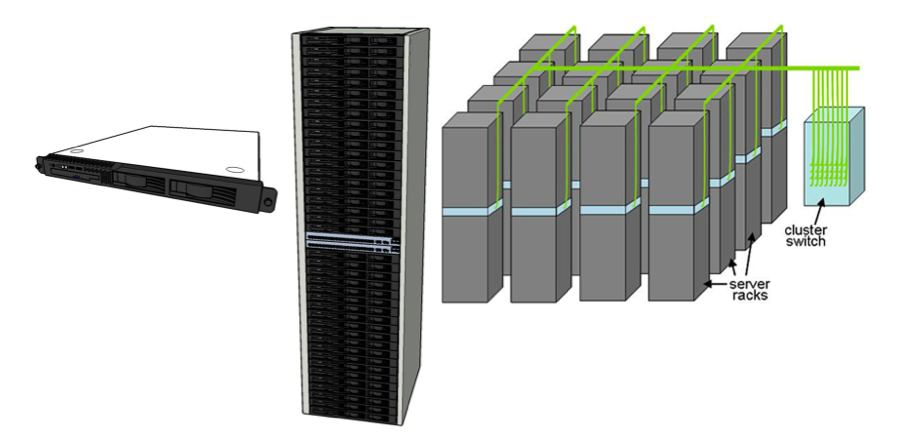
\includegraphics[width=0.7\textwidth]{images/racks} 
\caption{Organisation de racks.}
\end{center}
\end{figure}

L'image ci-dessus montre l'organisation des racks dans un data centre. Un serveur occupe 1 U du rack est montré à gauche. Au milieu on affiche un rack et à droite un cluster de racks avec un swtich/routeur de niveau cluster. En général un ensemble de serveurs 1U sont montés dans un rack et inter-connectés avec commutateur Ethernet local. Ces switches au niveau des racks, qui peuvent utiliser des liens de 1 à 10 Gbps, ont un nombre de connexions uplink vers un ou plus switches de niveau cluster (data centre).

Le stockage dans les data centre peut être fourni en diverses manières. Souvent le stockage de haute performance est logé dans des \og  tours de stockage \fg{} qui permettent un accès distant transparent au stockage indépendamment du nombre et des types des dispositifs de stockage physiques installés. Le stockage peut également être fourni dans  plus petit \og  brique de stockage \fg{} localisé dans le rack ou slot de chassis ainsi que directement intégré aux serveurs. Dans tous les cas, un accès réseau efficace au stockage est crucial.

Le problème le plus important dans cette structure est la potentielle insuffisance de bande passante. En général, les connexions uplink sont conçues pour supporter un certain taux de 
demande excédentaire puisque la fourniture d'une bande passante entière n'est toujours possible. Par exemple, 20 serveurs à 1Gbps chacun doit partagé un uplink Ethernet unique de 10Gps à un taux de demande excédentaire de 2. Cette situation peut être problématique si la charge réseau non local monte considérablement. Comme le stockage est traditionnellement fourni dans une tour séparée, tout le trafic de stockage traverse le lien uplink dans le réseau stockage. Par exemple, l'archivage d'un gros volume peut consommer une importante bande passante. À mesure que les data centres augmentent en taille, une architecture réseau plus extensible devient essentiel.

La consommation d'énergie constitue également des préoccupations à la conception des data centres car les coûts liés sont devenus un important composant de la totalité des coûts dette classe de systèmes. Actuellement le CPUs ne sont plus le seul élément cible d'amélioration de l'efficacité énergétique, vu qu'ils ne dominent plus la majorité de la consommation. Des problématiques de ventilation et surconsommation d'énergie sont de facteurs de plus en plus critiques de la conception de data centres.


\section{Virtualisation}

Virtualization refers to the abstraction of logical resources away from their underlying physical resources to improve agility and flexibility, reduce costs, and thus enhance business value. Virtualization allows a set of underutilized physical infrastructure components to be consolidated into a smaller number of better utilized devices, contributing to significant cost savings.

Server virtualization is a method of abstracting the operating system from the hardware platform. This allows multiple operating systems or multiple instances of the same operating system to coexist on one or more processors. A hypervisor or virtual machine monitor (VMM) is inserted between the operating system and the hardware to achieve this separation. These operating systems are called “guests” or “guest OSs.” The hypervisor provides hardware emulation to the guest operating systems. It also manages allocation of hardware resources between operating systems.


Integrated infrastructure solutions are specifically designed to provide advantages compared to a conventional physical infrastructure because they are: 
•	 Efficient in power usage, space utilization and IT employee productivity
•	 Economical in initial cost by making use of existing infrastructure and not requiring expensive room upgrades
•	 Interoperable through simplified design and implementation of systems and components 
•	 Controllable through planning, monitoring and management over the changing IT environment

\section{Technologies Associées}

\section{Principaux Challenges}

%According to a recent Gartner study, the leading challenges facing today’s data centers are intrinsic to many of the aforementioned business drivers and their associated IT solutions. Top challenges cited include: 
%• Keeping up with data growth 
%• Maintaining system performance and scalability
%• Mitigating network congestion and connectivity issues
%• Minimizing power, cooling and space costs
%• Effectively managing the data center and its infrastructure
%Furthermore, according to a 2011 survey of the Data Center Users’ Group (DCUG), the leading infrastructure challenges included data center availability, high heat densities, energy efficiency and maintaining adequate power densities (see Figure 1). Each of these challenges resonates closely with the leading data center challenges faced by IT professionals.

\section{Tendances des meilleures pratiques}

\subsection{Énergie}
1. Maximize the return temperature at the cooling units to improve capacity and efficiency
2. Match cooling capacity and airflow with IT loads
3. Utilize cooling designs that reduce energy consumption
4. Select a power system to optimize your availability and efficiency needs
5. Design for flexibility using scalable architectures that minimizes footprint

%Integrated infrastructure solutions are specifically designed to provide advantages compared to a conventional physical infrastructure because they are: 
%•	 Efficient in power usage, space utilization and IT employee productivity
%•	 Economical in initial cost by making use of existing infrastructure and not requiring expensive room upgrades
%•	 Interoperable through simplified design and implementation of systems and components 
%•	 Controllable through planning, monitoring and management over the changing IT environment
\section{Architecture}

\section{Cloud Computing}

Information technology (IT) is at a breaking point, and there is a critical need to improve IT's impact on the business.9
Consider the following:
 -As much as 85\% of computing capacity sits idle in distributed computing environments.
 -Seventy percent of IT budgets is typically spent on maintaining current IT infrastructures, and only 30\% is typically spent on new capabilities.
 -Over 30\% of consumers notified of a security breach will terminate their relationship with the company that contributed to the breach.
Clearly, infrastructures need to be more dynamic to free up budgets for new investments and accelerate deployment of superior capabilities being demanded by the business. Nearly all CEOs are adapting business models; cloud adoption can support these changing business dynamics.

Functional Areas in the Cloud-Ready Data Center
• Network Infrastructure—provides connectivity and transport for applications and services between users and the data center, within the data center and across multiple data centers. The Network infrastructure has three main sub components, namely the access network, the core network and the edge network.
• Compute and Storage—represents the compute and storage infrastructure appropriate for applications (rack-mount and chassis-based, cost-effective and multi-core, with unstructured content and highly structured transaction databases). The compute and storage functional area hosts all business applications such as Enterprise Resource Planning (ERP), SaaS, SOA and Web 2.0 applications (among others).
• Services—supports applications with security, user verification, and entitlement, and application support, including application acceleration, deep packet inspection (DPI), and load balancing
• Management and Orchestration—ties together all of the elements of the cloud-computing infrastructure, enabling efficient and responsive monitoring, management, and planning
